The $\ttbar+\ge 1c$ cross section, which is the nuisance parameter with high ranking and large constraint in the blinded fit, is found to have opposite pulls between 1L and 2LOS channel (see Figures \ref{fig:data_NP_ttbar}). Three follow-up studies are implemented to have a better understanding of this behavior.

First, Figure \ref{fig:TTC_deco_channels} shows the $\ttbar+\ge 1c$ cross section uncertainty decorrelated in each analysis region to see the pull effect in each region. Most of the regions in 1L channel with large statistic pull to 1$\sigma$ and most of the regions in 2LOS channel pull to -1$\sigma$. Figure \ref{fig:TTC_deco_combined} shows the combined fit comparison between the baseline fit and the fit with decorrelated $\ttbar+\ge 1c$ cross section uncertainty. No significant difference is found on other NPs. The correlation matrix of the combined fit with decorrelated $\ttbar+\ge 1c$ cross section uncertainty is shown in Figure \ref{fig:Corr_deco_TTC}.

Second, the $\ttbar+\ge 1c$ cross section uncertainty is fixed to 0 for individual fits on each channel. Figure \ref{fig:TTC_zero_1L} shows the NP pulls and constraints comparison among the baseline fit on 1L region, the fit with $\ttbar+\ge 1c$ cross section uncertainty fixed to 0 on 1L region and the baseline combined fit. Figure \ref{fig:TTC_zero_2L} shows the same comparison on 2LOS channel. No significant change is found in the case when $\ttbar+\ge 1c$ cross section uncertainty fixed to 0.

Finally, the $\ttbar+light$ cross section in 1L and 2LOS channel was decorrelated to make the fit behave well when deriving the HF rescaling factors. However, no dedicated NP is defined to control the $\ttbar+light$ normolisation. So an overall 50\% $\ttbar+light$ cross section is defined to see its tension on $\ttbar+\ge 1c$ cross section uncertainty. Figure \ref{fig:Corr_TTL} shows the correlation matrix of the combined fit with $\ttbar+light$ cross section uncertainty. The $\ttbar+light$ cross section uncertainty is highly correlated with $\ttbar+\ge 1c$ cross section uncertainty. Figure \ref{fig:TTL_combined} shows the NP pulls and constraint comparison between baseline combined fit and fit includes the $\ttbar+light$ cross section uncertainty and Figure \ref{fig:TTL_channels} shows the NPs of the fit includes the $\ttbar+light$ cross section uncertainty in 1L, 2LOS and combined channels. Even with a 50\% uncertainty on $\ttbar+light$ cross section, the impact is negligible and it cannot help to absorb the opposite pulls of $\ttbar+\ge 1c$ cross section uncertainty.

\begin{figure}[htbp!]
  \centering
  \begin{subfigure}[t]{0.32\textwidth}
    
\includegraphics[width=\linewidth]{figures/TTC_pull/deco_ch/NuisPar_comp_ttbar.pdf}
    \subcaption{\ttbar}
    \label{fig:TTC_deco_channels_ttbar}
  \end{subfigure}
  \begin{subfigure}[t]{0.32\textwidth}
    
\includegraphics[width=\linewidth]{figures/TTC_pull/deco_ch/NuisPar_comp_Instrumental.pdf}
    \subcaption{Instrumental}
    \label{fig:TTC_deco_channels_Instrumental}
  \end{subfigure}
  \begin{subfigure}[t]{0.32\textwidth}
    
\includegraphics[width=\linewidth]{figures/TTC_pull/deco_ch/NuisPar_comp_Other.pdf}
    \subcaption{Other}
    \label{fig:TTC_deco_channels_Other}
  \end{subfigure}
  \caption{\label{fig:TTC_deco_channels}NPs comparison among the fits with decorelated $\ttbar+\ge 1c$ cross section uncertainty on 1L, 2L and combined channels.}
\end{figure}

\begin{figure}[htbp!]
  \centering
  \begin{subfigure}[t]{0.32\textwidth}
    
\includegraphics[width=\linewidth]{figures/TTC_pull/deco_combined/NuisPar_comp_ttbar.pdf}
    \subcaption{\ttbar}
    \label{fig:TTC_deco_combined_ttbar}
  \end{subfigure}
  \begin{subfigure}[t]{0.32\textwidth}
    
\includegraphics[width=\linewidth]{figures/TTC_pull/deco_combined/NuisPar_comp_Instrumental.pdf}
    \subcaption{Instrumental}
    \label{fig:TTC_deco_combined_Instrumental}
  \end{subfigure}
  \begin{subfigure}[t]{0.32\textwidth}
    
\includegraphics[width=\linewidth]{figures/TTC_pull/deco_combined/NuisPar_comp_Other.pdf}
    \subcaption{Other}
    \label{fig:TTC_deco_combined_Other}
  \end{subfigure}
  \caption{\label{fig:TTC_deco_combined}NPs comparison between the baseline combined fit and combined fit with decorelated $\ttbar+\ge 1c$ cross section uncertainty.}
\end{figure}

\begin{figure}[htbp!]
        \centering
        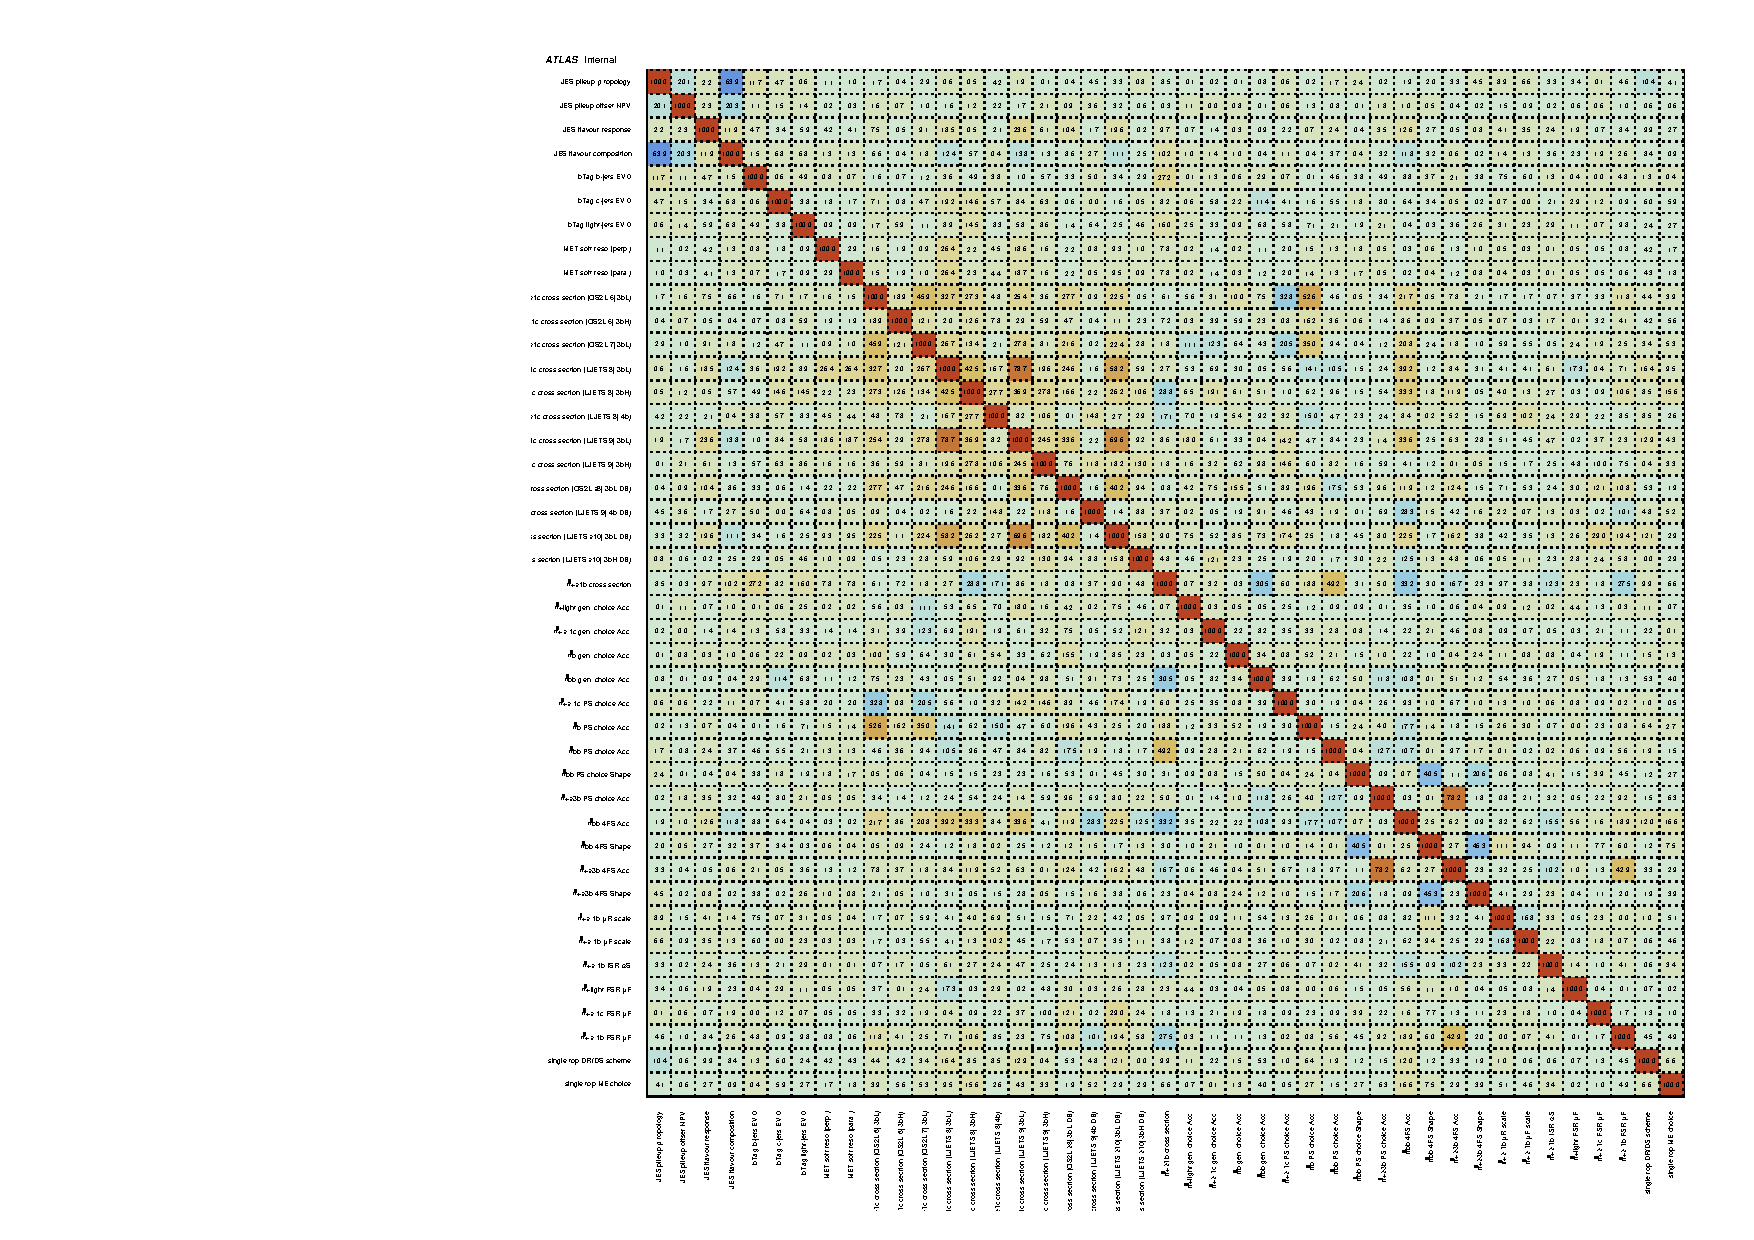
\includegraphics[width=\linewidth]{figures/TTC_pull/corr_matrix/CorrMatrix_decorrelated_TTC.pdf}
        \caption{\label{fig:Corr_deco_TTC}Correlation matrix combined fit with decorelated $\ttbar+\ge 1c$ cross section uncertainty.}
\end{figure}

\begin{figure}[htbp!]
  \centering
  \begin{subfigure}[t]{0.32\textwidth}
    
\includegraphics[width=\linewidth]{figures/TTC_pull/zero_1L/NuisPar_comp_ttbar.pdf}
    \subcaption{\ttbar}
    \label{fig:TTC_zero_1L_ttbar}
  \end{subfigure}
  \begin{subfigure}[t]{0.32\textwidth}
    
\includegraphics[width=\linewidth]{figures/TTC_pull/zero_1L/NuisPar_comp_Instrumental.pdf}
    \subcaption{Instrumental}
    \label{fig:TTC_zero_1L_Instrumental}
  \end{subfigure}
  \begin{subfigure}[t]{0.32\textwidth}
    
\includegraphics[width=\linewidth]{figures/TTC_pull/zero_1L/NuisPar_comp_Other.pdf}
    \subcaption{Other}
    \label{fig:TTC_zero_1L_Other}
  \end{subfigure}
  \caption{\label{fig:TTC_zero_1L}NPs comparison among the baseline fit on 1L region, the fit with $\ttbar+\ge 1c$ cross section uncertainty fixed to 0 on 1L region and baseline combined fit.}
\end{figure}

\begin{figure}[htbp!]
  \centering
  \begin{subfigure}[t]{0.32\textwidth}
    
\includegraphics[width=\linewidth]{figures/TTC_pull/zero_1L/NuisPar_comp_ttbar.pdf}
    \subcaption{\ttbar}
    \label{fig:TTC_zero_2L_ttbar}
  \end{subfigure}
  \begin{subfigure}[t]{0.32\textwidth}
    
\includegraphics[width=\linewidth]{figures/TTC_pull/zero_1L/NuisPar_comp_Instrumental.pdf}
    \subcaption{Instrumental}
    \label{fig:TTC_zero_2L_Instrumental}
  \end{subfigure}
  \begin{subfigure}[t]{0.32\textwidth}
    
\includegraphics[width=\linewidth]{figures/TTC_pull/zero_1L/NuisPar_comp_Other.pdf}
    \subcaption{Other}
    \label{fig:TTC_zero_2L_Other}
  \end{subfigure}
  \caption{\label{fig:TTC_zero_2L}NPs comparison among the baseline fit on 2L region, the fit with $\ttbar+\ge 1c$ cross section uncertainty fixed to 0 on 2L region and baseline combined fit.}
\end{figure}

\begin{figure}[htbp!]
        \centering
        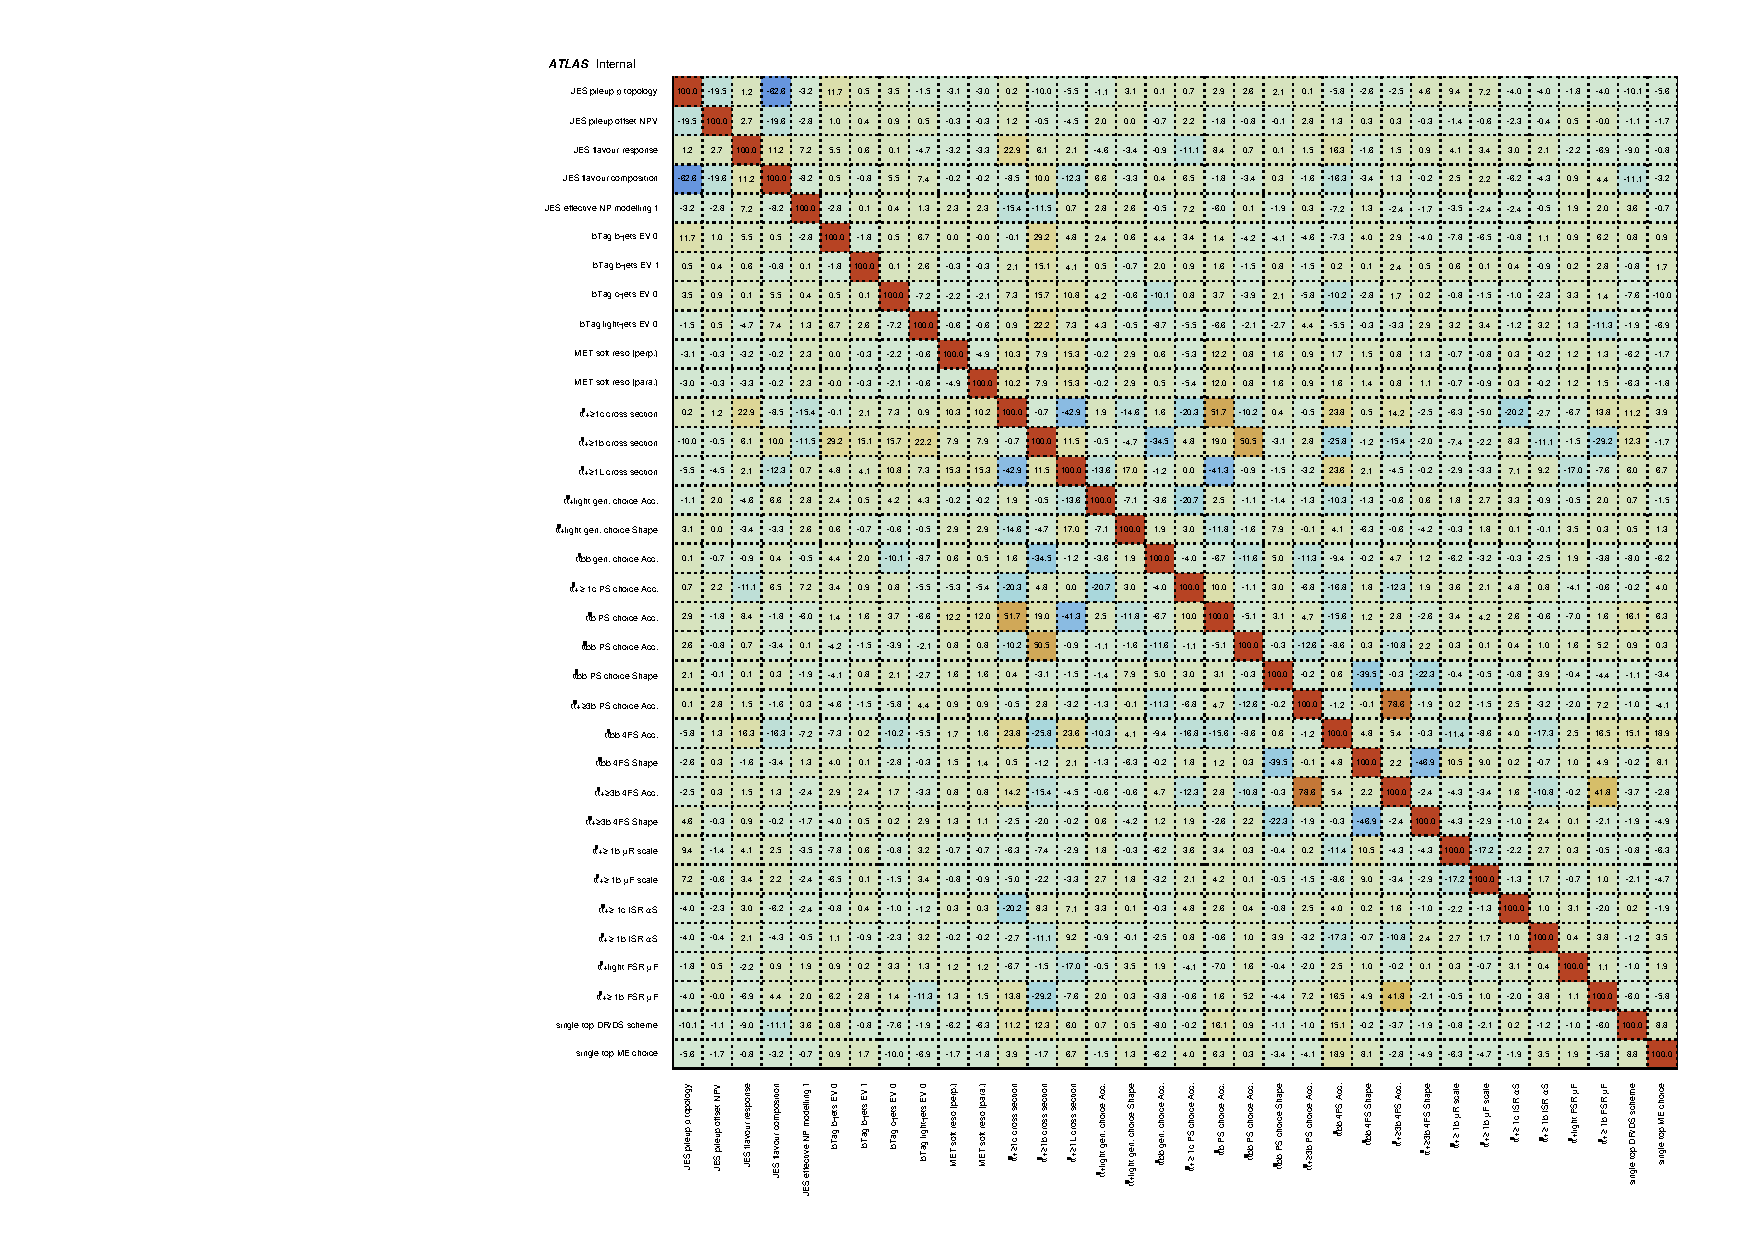
\includegraphics[width=\linewidth]{figures/TTC_pull/corr_matrix/CorrMatrix_TTL_all.pdf}
        \caption{\label{fig:Corr_TTL}Correlation matrix combined fit inclueds $\ttbar+light$ cross section uncertainty.}
\end{figure}


\begin{figure}[htbp!]
  \centering
  \begin{subfigure}[t]{0.32\textwidth}
    
\includegraphics[width=\linewidth]{figures/TTC_pull/TTL_combined/NuisPar_comp_ttbar.pdf}
    \subcaption{\ttbar}
    \label{fig:TTL_combined_ttbar}
  \end{subfigure}
  \begin{subfigure}[t]{0.32\textwidth}
    
\includegraphics[width=\linewidth]{figures/TTC_pull/TTL_combined/NuisPar_comp_Instrumental.pdf}
    \subcaption{Instrumental}
    \label{fig:TTL_combined_Instrumental}
  \end{subfigure}
  \begin{subfigure}[t]{0.32\textwidth}
    
\includegraphics[width=\linewidth]{figures/TTC_pull/TTL_combined/NuisPar_comp_Other.pdf}
    \subcaption{Other}
    \label{fig:TTL_combined_Other}
  \end{subfigure}
  \caption{\label{fig:TTL_combined}NPs comparison between the baseline combined fit and combined fit includes $\ttbar+light$ cross section uncertainty.}
\end{figure}

\begin{figure}[htbp!]
  \centering
  \begin{subfigure}[t]{0.32\textwidth}
    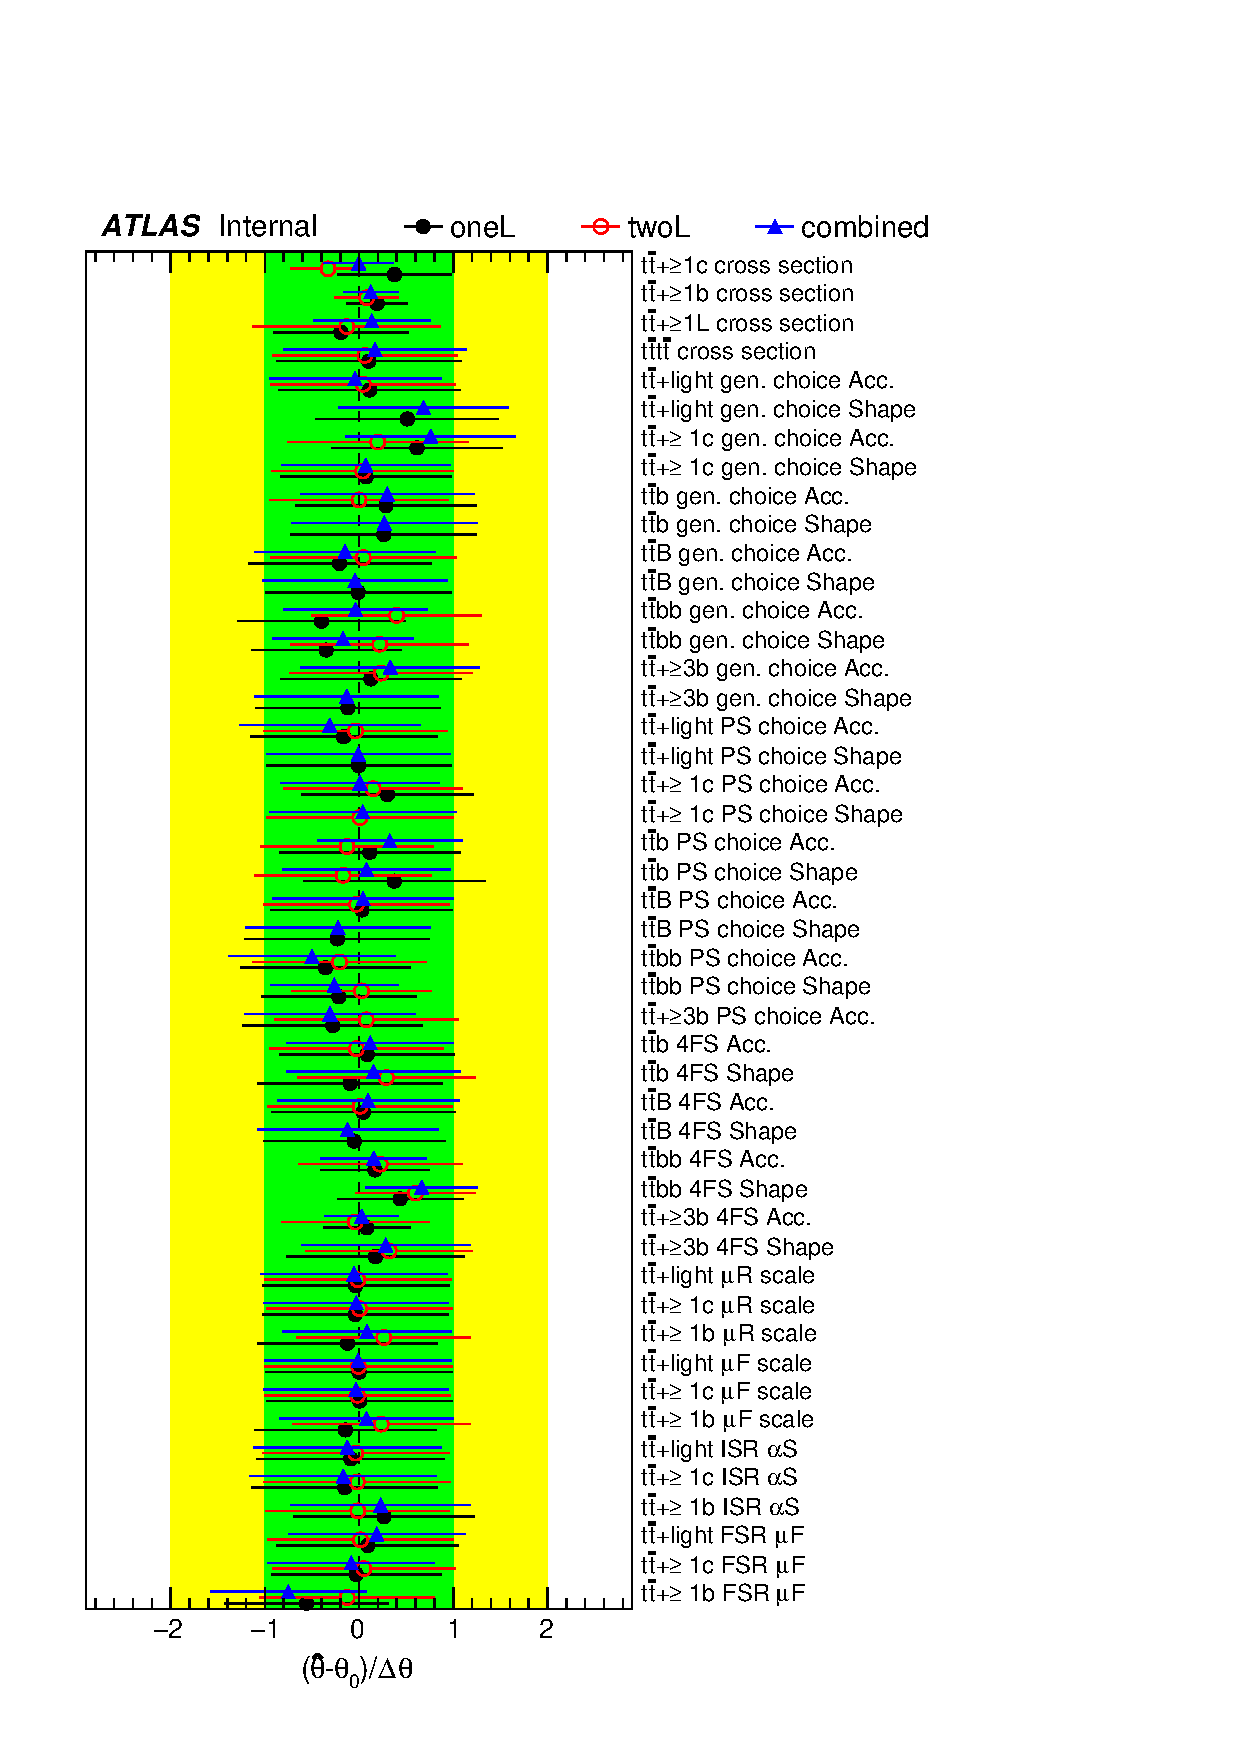
\includegraphics[width=\linewidth]{figures/TTC_pull/TTL_ch/NuisPar_comp_ttbar.pdf}
    \subcaption{\ttbar}
    \label{fig:TTL_channels_ttbar}
  \end{subfigure}
  \begin{subfigure}[t]{0.32\textwidth}
    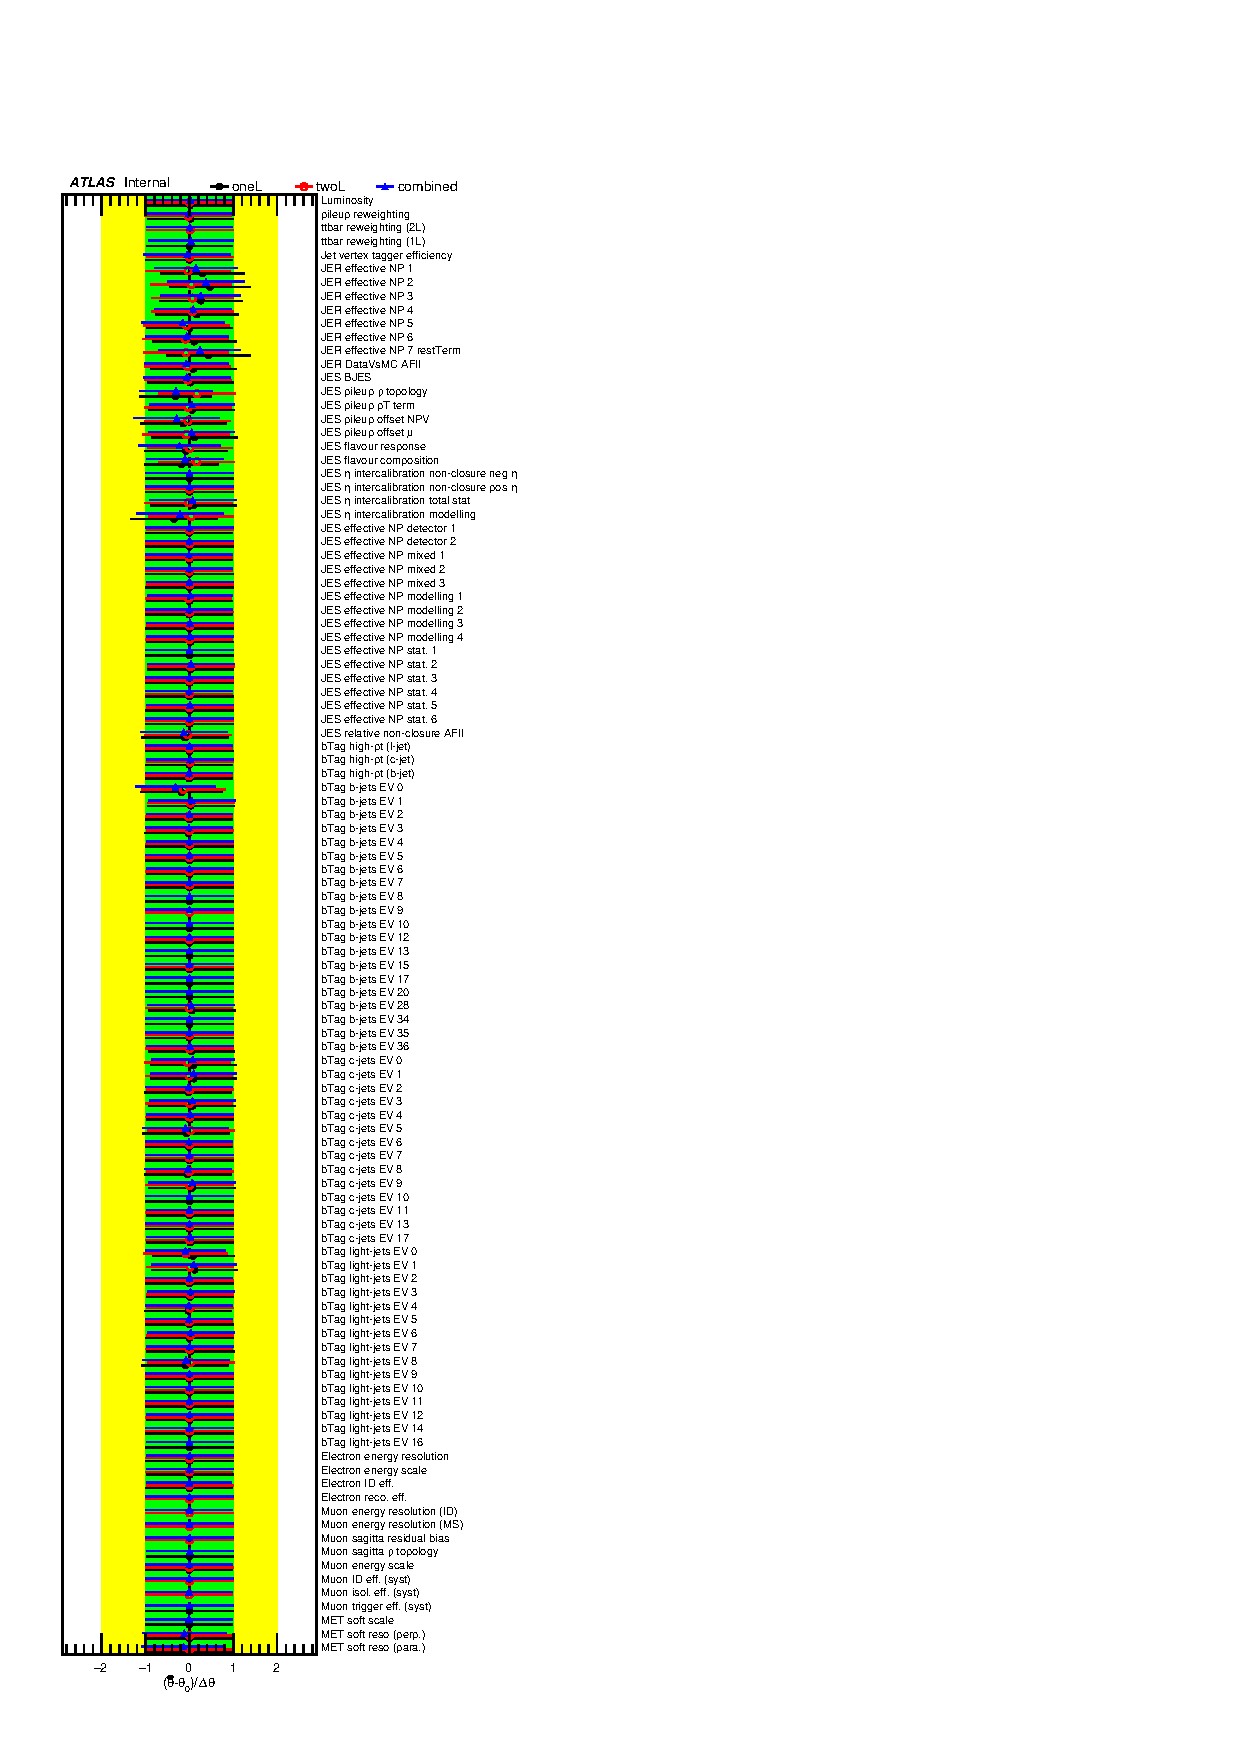
\includegraphics[width=\linewidth]{figures/TTC_pull/TTL_ch/NuisPar_comp_Instrumental.pdf}
    \subcaption{Instrumental}
    \label{fig:TTL_channels_Instrumental}
  \end{subfigure}
  \begin{subfigure}[t]{0.32\textwidth}
    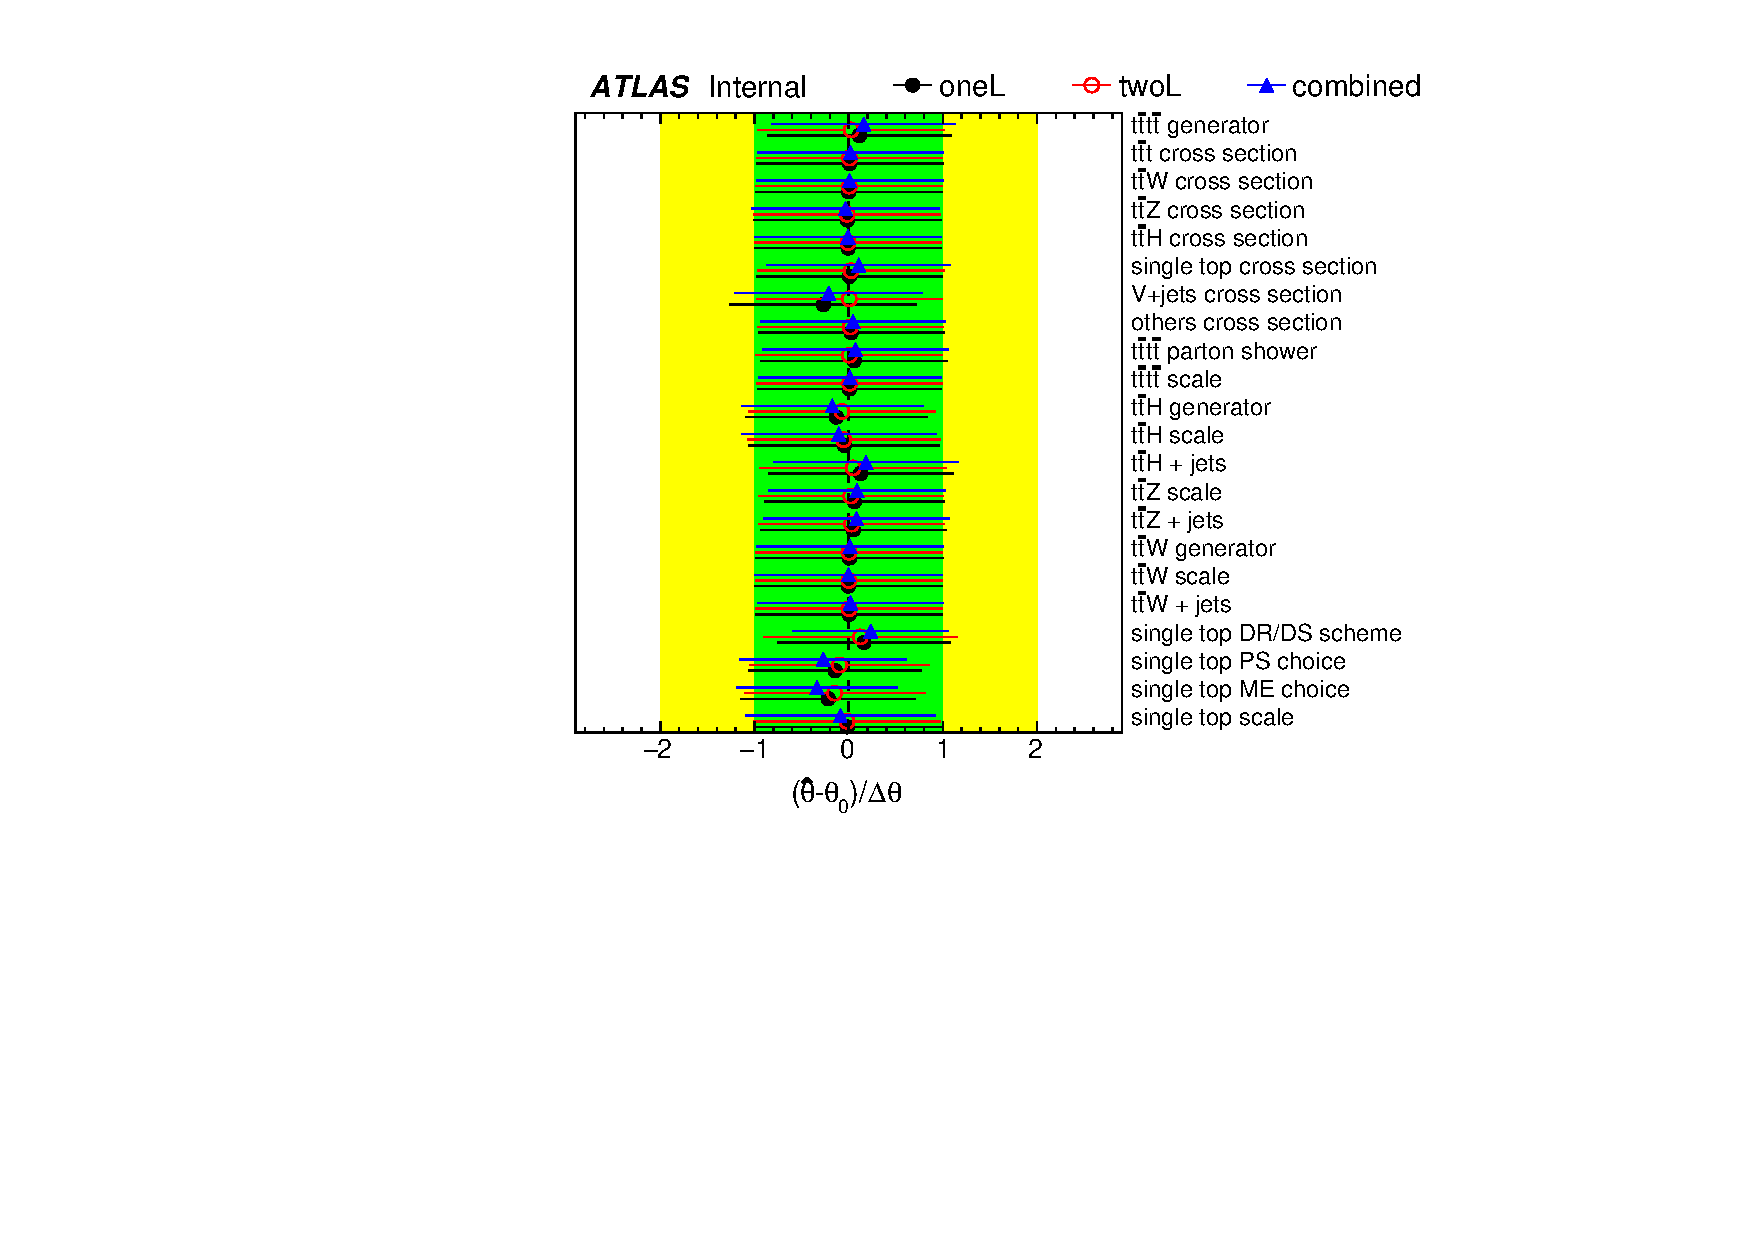
\includegraphics[width=\linewidth]{figures/TTC_pull/TTL_ch/NuisPar_comp_Other.pdf}
    \subcaption{Other}
    \label{fig:TTL_channels_Other}
  \end{subfigure}
  \caption{\label{fig:TTL_channels}NPs comparison among the fits includes $\ttbar+light$ cross section uncertainty on 1L, 2L and combined channels.}
\end{figure}
\clearpage


\subsection{TTC Normalisation Uncertainty}
The following subsection shows $\ttbar+\ge 1c$ normalisation uncertainty effect on overall MC compared to data for GNN discriminant for masspoint 400 in single lepton and dilepton opposite sign channel. 

\begin{figure}[htpb!]

        \begin{center} \setlength{\tabcolsep}{2.5pt}\footnotesize
        \begin{tabular}{cccc} 
        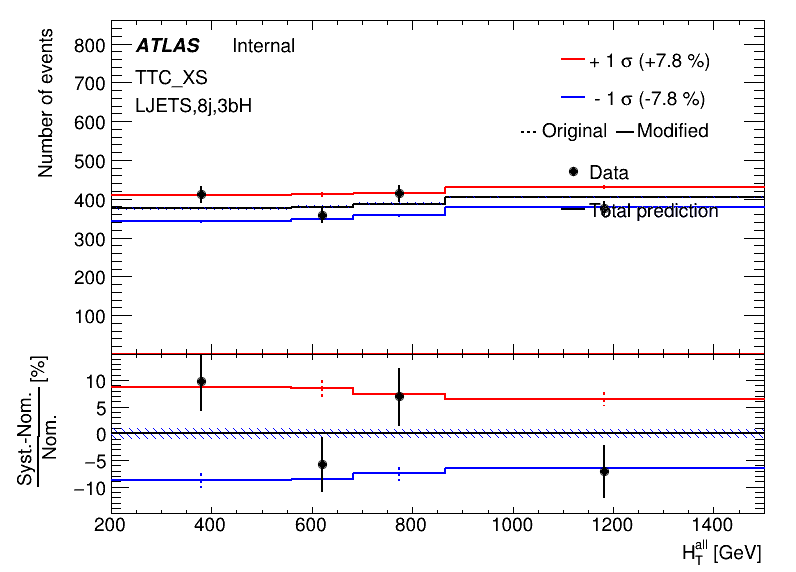
\includegraphics[width=0.3 \textwidth]{figures/TTC_pull/TTC_XS/ljets_8j3bH_Combined_TTC_XS.png} &
        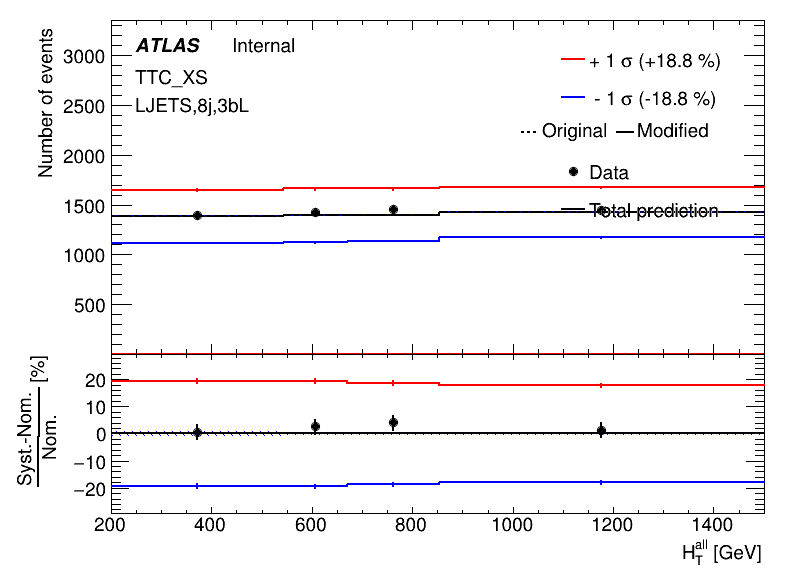
\includegraphics[width=0.3 \textwidth]{figures/TTC_pull/TTC_XS/ljets_8j3bL_Combined_TTC_XS.png} &
        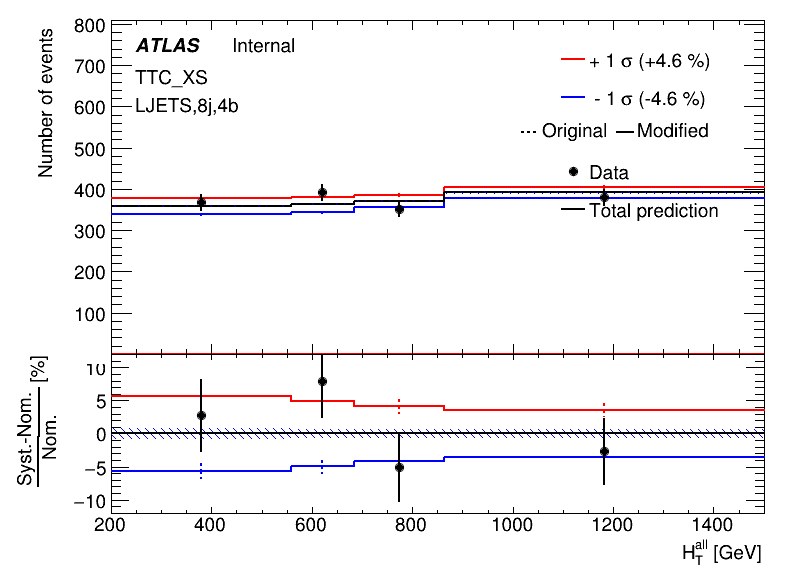
\includegraphics[width=0.3 \textwidth]{figures/TTC_pull/TTC_XS/ljets_8j4b_Combined_TTC_XS.png}\\

        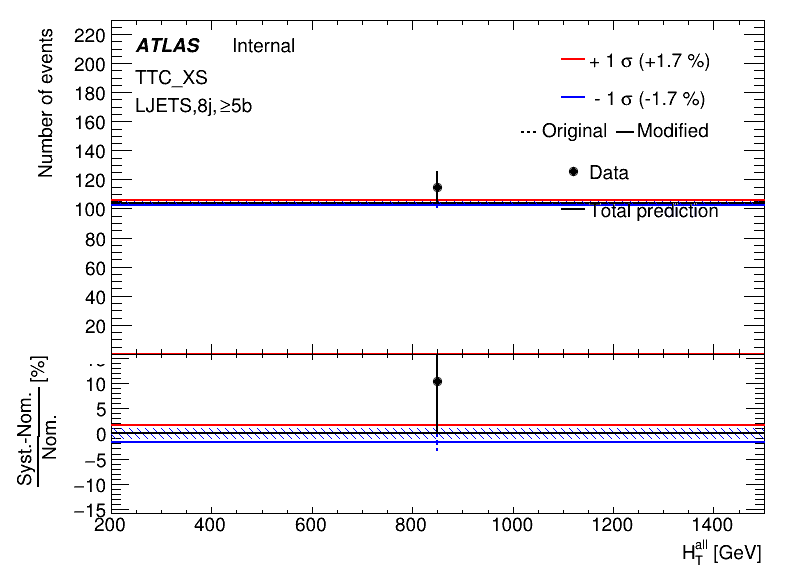
\includegraphics[width=0.3 \textwidth]{figures/TTC_pull/TTC_XS/ljets_8jge5b_Combined_TTC_XS.png} &                                                 
        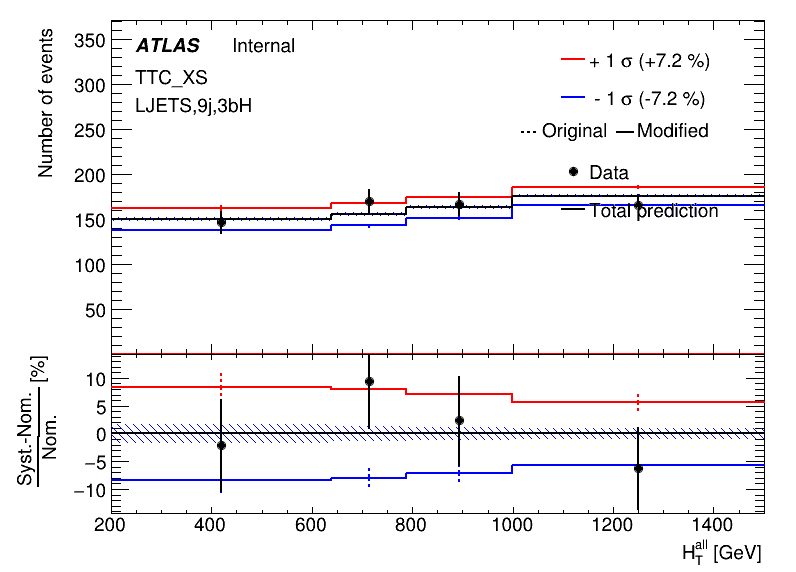
\includegraphics[width=0.3 \textwidth]{figures/TTC_pull/TTC_XS/ljets_9j3bH_Combined_TTC_XS.png} &                                                  
        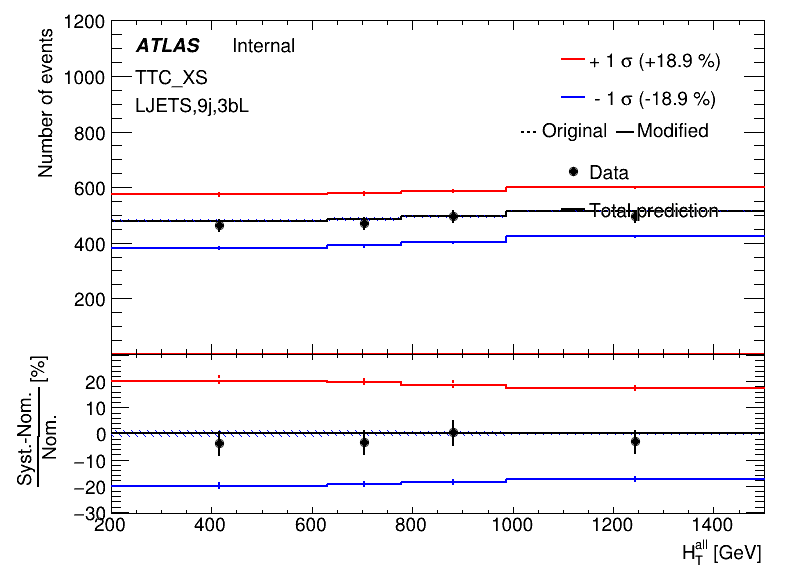
\includegraphics[width=0.3 \textwidth]{figures/TTC_pull/TTC_XS/ljets_9j3bL_Combined_TTC_XS.png}\\ 
        
        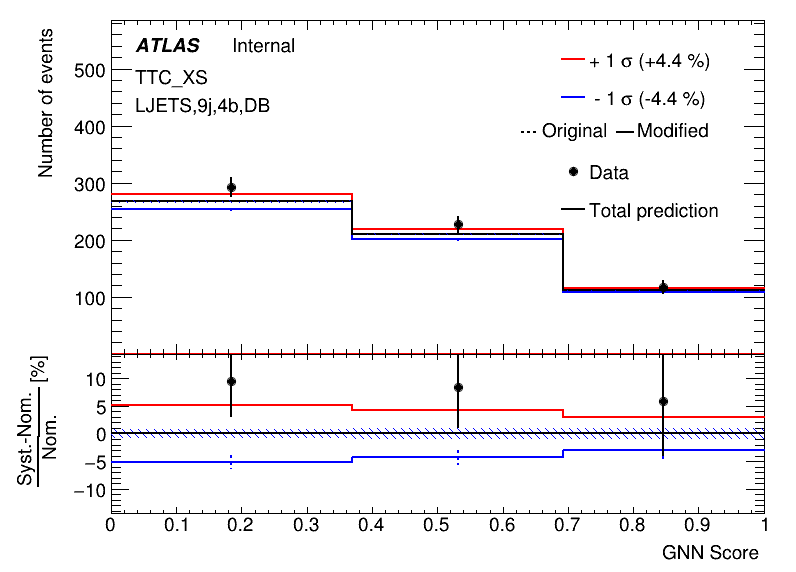
\includegraphics[width=0.3 \textwidth]{figures/TTC_pull/TTC_XS/ljets_9j4b_DB_Combined_TTC_XS.png} &                                                   
        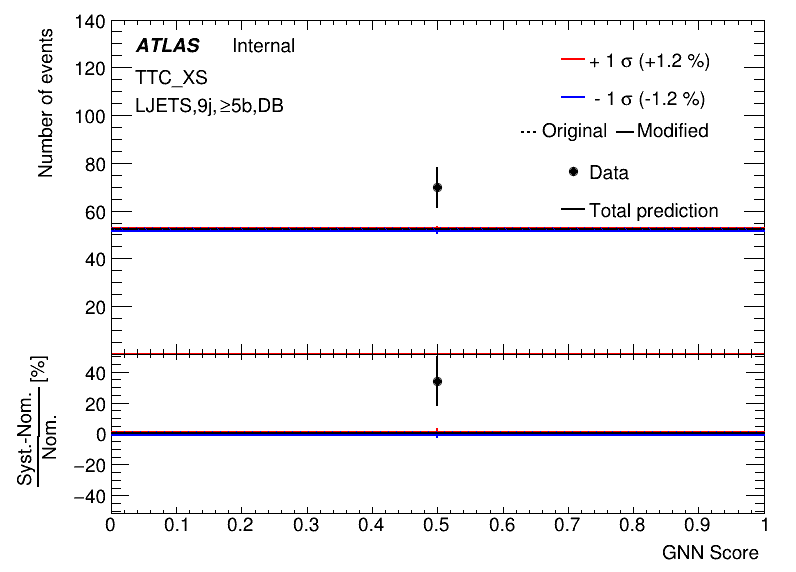
\includegraphics[width=0.3 \textwidth]{figures/TTC_pull/TTC_XS/ljets_9jge5b_DB_Combined_TTC_XS.png} &                                                 
        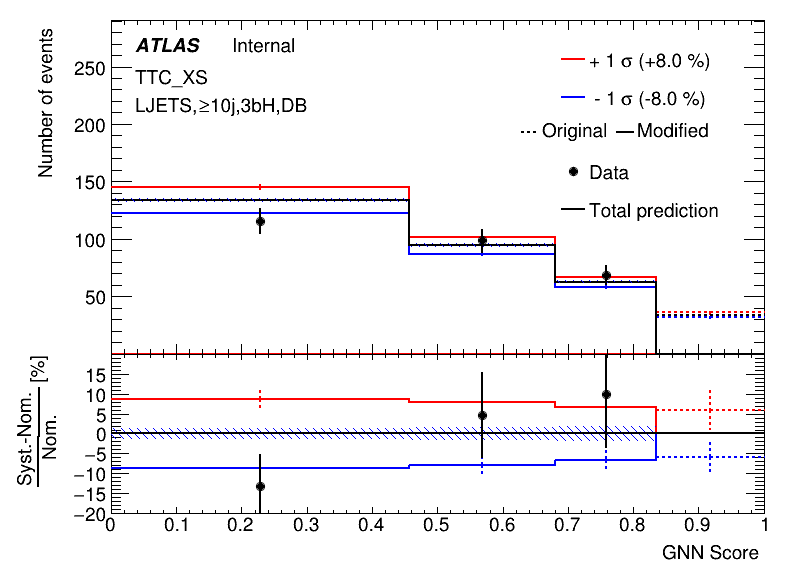
\includegraphics[width=0.3 \textwidth]{figures/TTC_pull/TTC_XS/ljets_ge10j3bH_DB_Combined_TTC_XS.png}\\    

        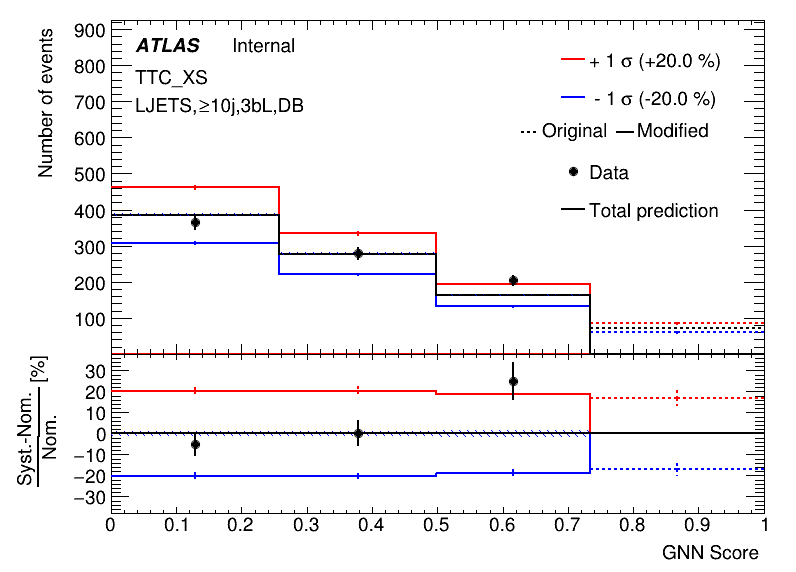
\includegraphics[width=0.3 \textwidth]{figures/TTC_pull/TTC_XS/ljets_ge10j3bL_DB_Combined_TTC_XS.png} &                                               
        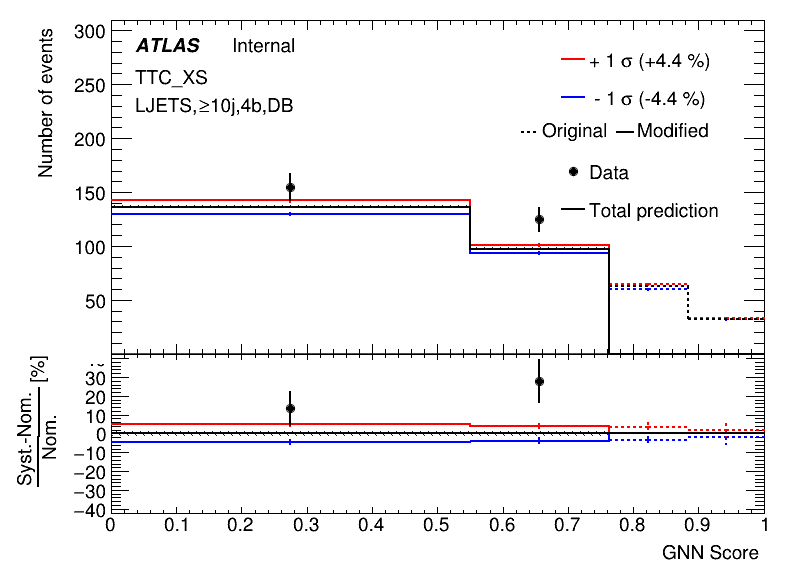
\includegraphics[width=0.3 \textwidth]{figures/TTC_pull/TTC_XS/ljets_ge10j4b_DB_Combined_TTC_XS.png} &                                                
        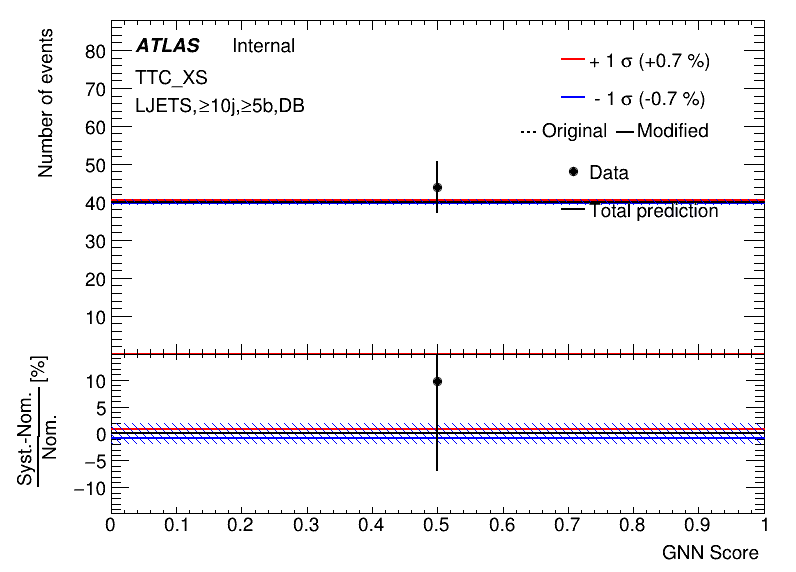
\includegraphics[width=0.3 \textwidth]{figures/TTC_pull/TTC_XS/ljets_ge10jge5b_DB_Combined_TTC_XS.png}\\ 
        
        \end{tabular}                                                                                                                                   
        \end{center}  
        
        \caption{\label{TTC_XS_Uncertainty_1L}The TTC normalisation  uncertainty red/blue plots for GNN400 in 1L channel are shown above.}


\end{figure}

\begin{figure}[htpb!]                                                                                                                                     
                                                                                                                                                          
  \begin{center} \setlength{\tabcolsep}{2.5pt}\footnotesize                                                                                           
        \begin{tabular}{cccc} 
        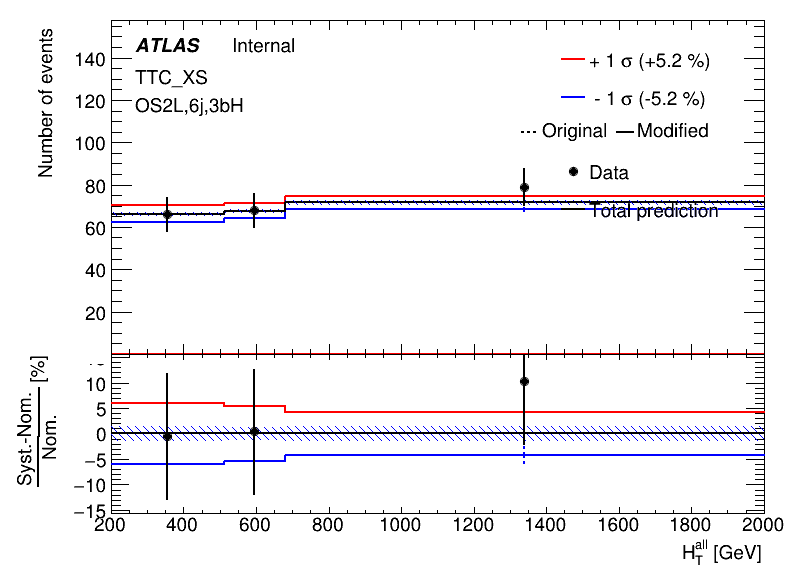
\includegraphics[width=0.3 \textwidth]{figures/TTC_pull/TTC_XS/os2l_6j3bH_Combined_TTC_XS.png} &                                                   
        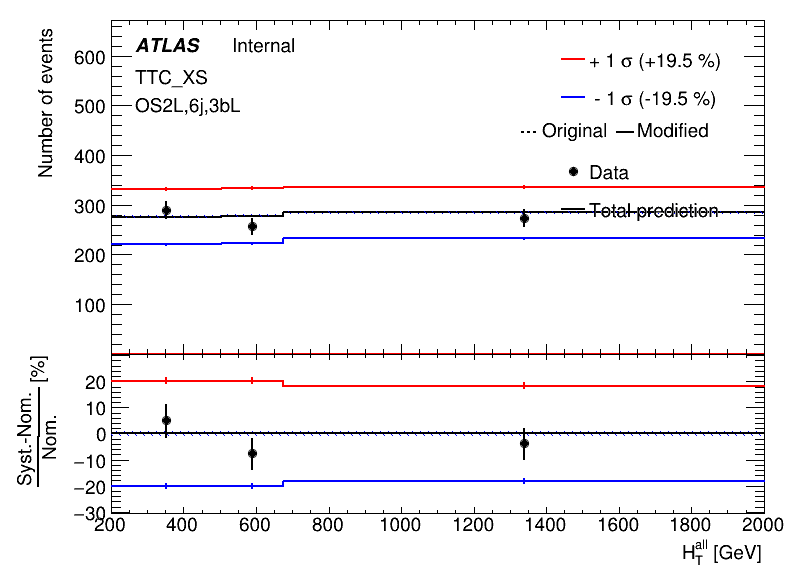
\includegraphics[width=0.3 \textwidth]{figures/TTC_pull/TTC_XS/os2l_6j3bL_Combined_TTC_XS.png} &                                                   
        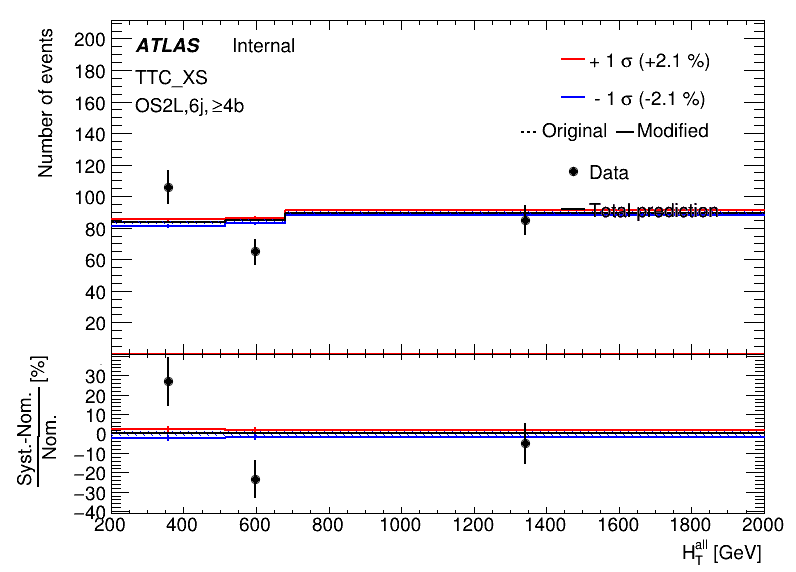
\includegraphics[width=0.3 \textwidth]{figures/TTC_pull/TTC_XS/os2l_6jge4b_Combined_TTC_XS.png}\\ 

        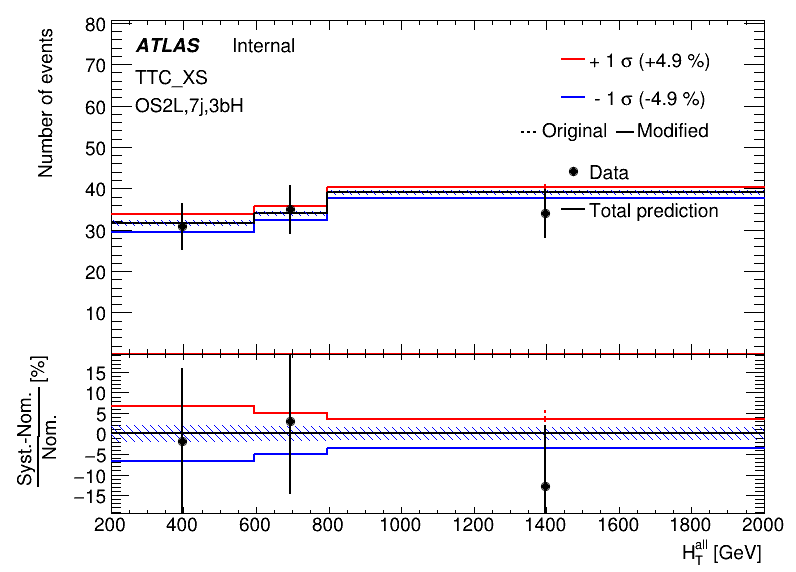
\includegraphics[width=0.3 \textwidth]{figures/TTC_pull/TTC_XS/os2l_7j3bH_Combined_TTC_XS.png} &                                                   
        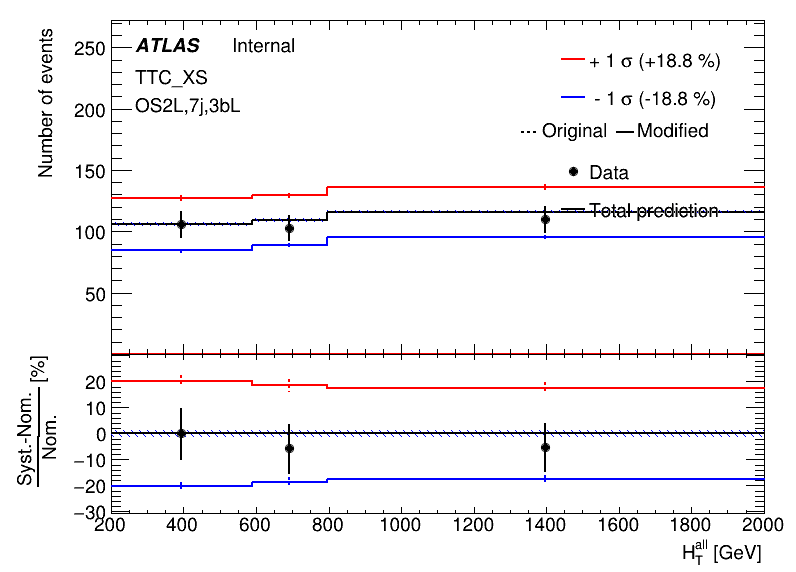
\includegraphics[width=0.3 \textwidth]{figures/TTC_pull/TTC_XS/os2l_7j3bL_Combined_TTC_XS.png} &                                             
        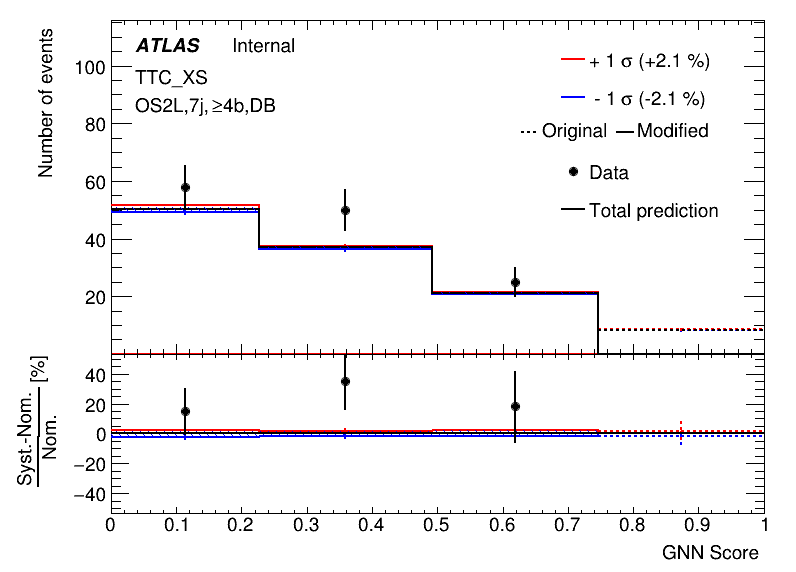
\includegraphics[width=0.3 \textwidth]{figures/TTC_pull/TTC_XS/os2l_7jge4b_DB_Combined_TTC_XS.png}\\
        
        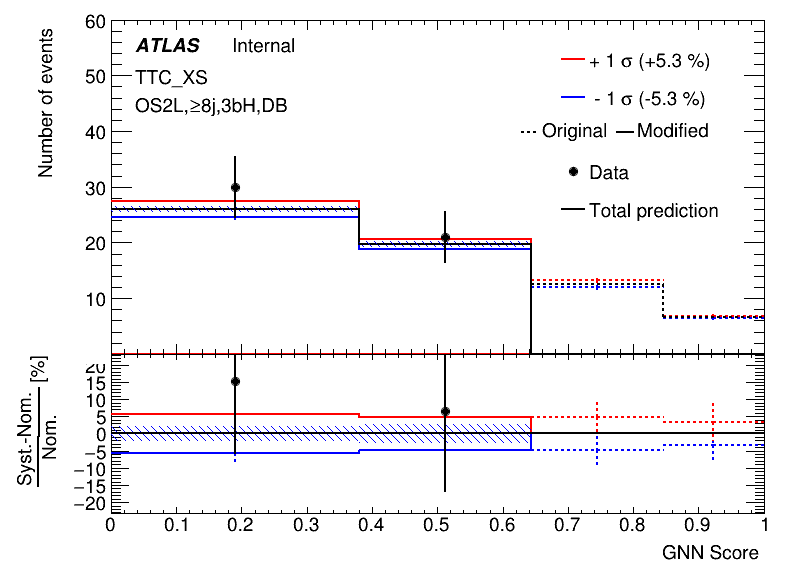
\includegraphics[width=0.3 \textwidth]{figures/TTC_pull/TTC_XS/os2l_ge8j3bH_DB_Combined_TTC_XS.png} &                                                 
        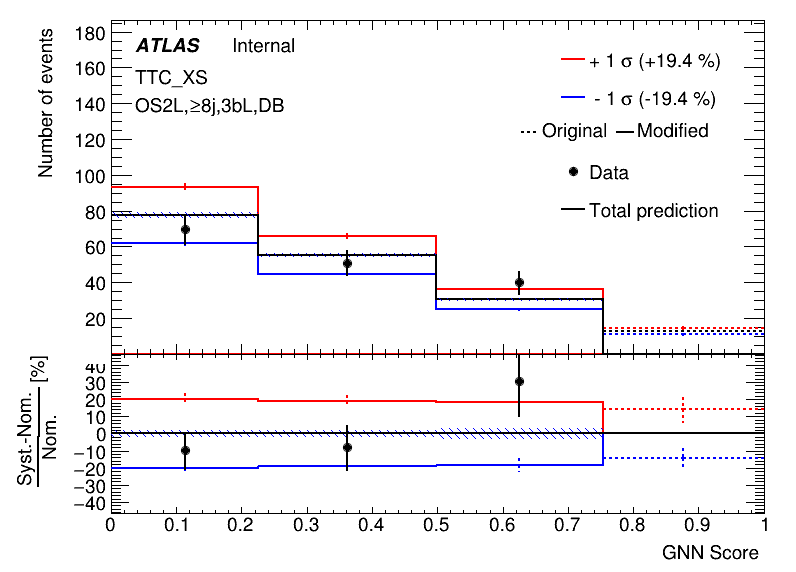
\includegraphics[width=0.3 \textwidth]{figures/TTC_pull/TTC_XS/os2l_ge8j3bL_DB_Combined_TTC_XS.png} &                                                 
        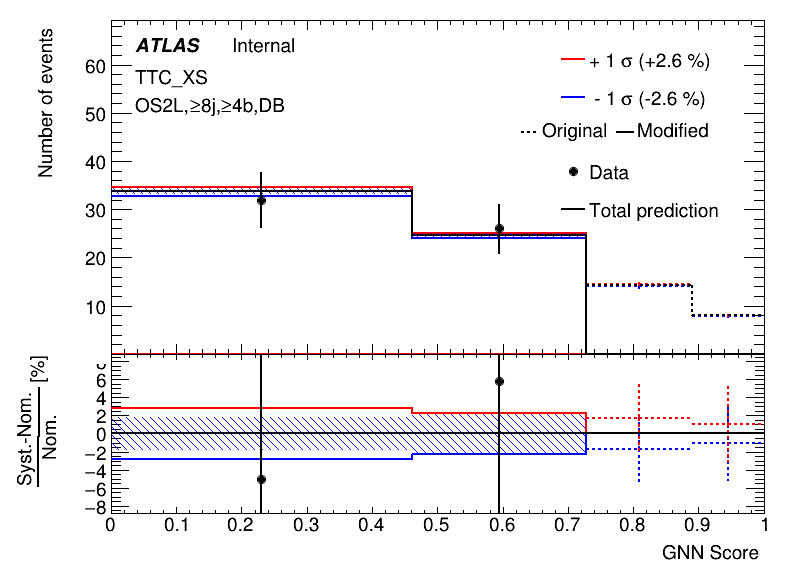
\includegraphics[width=0.3 \textwidth]{figures/TTC_pull/TTC_XS/os2l_ge8jge4b_DB_Combined_TTC_XS.png}\\ 

        \end{tabular}                                                                                                                                      
        \end{center}

        \caption{\label{TTC_XS_Uncertainty_2LOS}The TTC normalisation  uncertainty red/blue plots for GNN400 in 2LOS channel are shown above.}

\end{figure}
